\documentclass[nonacm, acmsmall, screen, 10pt]{acmart}

\usepackage{minted}

\setminted[java]{fontsize=\small, tabsize=2, breaklines, linenos}
\setminted[text]{fontsize=\small, tabsize=2, breaklines, linenos}
\setminted[gas]{fontsize=\small, tabsize=2, breaklines, linenos}
\setminted[c]{fontsize=\small, tabsize=2, breaklines, linenos}

\begin{document}
\title{CS4212 Programming Assignment 3 Report}
\author{Julius Putra Tanu Setiaji (A0149787E)}\makeatletter\let\@authorsaddresses\@empty\makeatother%
\maketitle
\tableofcontents

\section{Compiler Usage}
To compile a JLite source code into ARM assembly code without optimisation, run:
\begin{verbatim}
./jlitec arm <input file>
\end{verbatim}

To compile a JLite source code into ARM assembly code with optimisations run on the Lower IR as well as peephole optimisations on the ARM code, run:
\begin{verbatim}
./jlitec arm -O3 <input file>
\end{verbatim}

To compile a JLite source code into ARM assembly code with optimisations run on the Lower IR but without the peephole optimisations on the ARM code, run:
\begin{verbatim}
./jlitec arm -O2 <input file>
\end{verbatim}

\subsection{Using GCC to assemble the assembly source code}
Redirect the output of my compiler into a file, and then pass this file to a GCC (cross) compiler for ARM.
For example, if your input file is \texttt{a.j}, in \texttt{bash}, run:
\begin{verbatim}
./jlitec arm a.j > /tmp/a.s
case "$(uname -s)" in
  Linux*)  CC_ARM=arm-linux-gnueabihf-gcc;;
  Darwin*) CC_ARM=arm-unknown-linux-gnueabi-gcc;;
esac
[[ CC_ARM != "" ]] && $CC_ARM /tmp/a.s --static || echo Unknown platform
\end{verbatim}

\subsection{Using gem5 to run the output binary}
Assuming the output binary is in \texttt{/tmp/a.out}, change directory to where gem5 is located, then run:
\begin{verbatim}
./build/ARM/gem5.opt configs/example/se.py -c /tmp/a.out -i /dev/tty
\end{verbatim}

By specifying input file as \texttt{/dev/tty}, you can provide input to the resulting binary from \texttt{stdin} for any \texttt{readln} uses.

\section{General Compilation Flow}
Besides IR3, I defined my own machine-specific intermediate representation (IR) for use in my compiler, called Lower.
With reference to GCC, IR3 is similar to GIMPLE, while Lower is similar to RTL.

My compiler can be divided into several parts:
\begin{enumerate}
  \item Lexer
  \item Parser
  \item Typechecker
  \item IR3 Codegen
  \item Lower Codegen
  \item Optional optimisation passes
  \item Register Allocation
  \item ARM code generation
  \item Optional peephole optimisation passes
\end{enumerate}

\subsection{Lexer and Parser}
Lexer and parser were done as part of Programming Assignment 1.

Lexing is done using the lexer generator JFlex.
It was relatively straightforward as the tokens in JLite is a subset of the tokens in Java, and JFlex provided a sample Java lexer.
The one difference between Java tokens are JLite tokens is the liberty that I took to disallow representing the empty string as \texttt{""}, and instead forcing the use of \texttt{null} to represent empty string.

Parsing is done using the LALR parser generator CUP.
This part is more complicated as the provided grammar is ambiguous, due to the type-specificity of each operator, the overloading of the operator \texttt{+} to represent both arithmetic addition and string concatenation, and the associativity ambiguity of the string concatenation operator.
Thus, I specified a less strict grammar rules, and verified the abstract syntax tree during construction in order to make sure it follows the full JLite grammar rules.

The generated abstract syntax tree is then passed on to the typechecker.

\subsection{Typechecker and IR3 Codegen}
Typechecker and IR3 code generation were done as part of Programming Assignment 1.

Typechecking is performed on the abstract syntax tree recursively, and the types are attached to the abstract syntax tree.
My compiler supports function overloading based on types of the parameters of a method, together with a check that there is no two method with duplicate signature (defined as the types of the parameters).
The method resolution is then based on the types of the parameters to yield the correct return type for the method.

Generating IR3 from the abstract syntax tree is quite trivial through recursion with the information yielded from the typechecker, i.e. the type information and the method resolution information.
IR3 does not have a notion of classes anymore, only structs and functions that act on structs.
The generated IR3 code is then passed on to the Lower codegen.

\subsection{Lower Codegen}
Lower is my machine-specific where I perform all the passes on.
Unlike Jlite and IR3, Lower does not have any notion of expression, only statements.
These statements are designed to very closely match ARM instructions, while still maintaining IR3 semantics as much as possible to still allow reasonable optimization at this IR level.
Lower also allows statements to make use of real physical hardware ARM registers, besides variables.
The struct \texttt{Addressable} in Lower is designed to be the representation of a ``register'', both real physical hardware registers as well as pseudo-registers (which program variables are).

The pass that lowers IR3 to Lower is the file \texttt{LowerPass.java}.

There are many types of statements in Lower (located in \texttt{src/main/java/jlitec/\-backend/\-passes/\-lower/\-stmt/}):
\begin{itemize}
  \item \texttt{BINARY}, representing instructions in ARM whose operands are one register and one Operand2 that is either Immediate or Register without barrel-shifter operation.
  \item \texttt{BINARY\_BIT}, representing instructions in ARM whose operands are one register and one Register with barrel-shifter operation.
  \item \texttt{BIT}, representing barrel-shifter instructions in ARM.
  \item \texttt{BRANCH\_LINK}, representing the \texttt{BL} instruction.
  \item \texttt{CMP}, representing an if-goto instruction (\texttt{CMP} followed by conditional \texttt{B} instructions).
  \item \texttt{FIELD\_ACCESS}, representing a field access (\texttt{LDR} instruction).
  \item \texttt{FIELD\_ASSIGN}, representing a field assignment (\texttt{STR} instruction).
  \item \texttt{GOTO}, representing unconditional branching (unconditional \texttt{B} instruction).
  \item \texttt{IMMEDIATE}, representing assignment into a register from an immediate value (either \texttt{MOV} instruction with an immediate operand2, or \texttt{LDR} from a constant pool, as is the case for literal strings).
  \item \texttt{LABEL}, representing a label.
  \item \texttt{LOAD\_STACK\_ARG}, representing \texttt{LDR} instruction from the stack for a function argument.
  \item \texttt{LOAD\_LARGE\_IMM}, representing assignment into a register from the constant pool for a large immediate value.
  \item \texttt{LDR\_SPILL}, representing \texttt{LDR} instruction for a spilled variable.
  \item \texttt{STR\_SPILL}, representing \texttt{STR} instruction for a spilled variable.
  \item \texttt{MOV}, representing assignment from one register into another (\texttt{MOV} instruction with two register operands).
  \item \texttt{RETURN}, representing returning from the current function (either \texttt{BX LR} instruction or \texttt{LDMFD SP!, \{..., PC\}}).
  \item \texttt{PUSH\_PAD\_STACK}, representing \texttt{SUB SP, SP, \#4} to pad the stack by 4 bytes to maintain 8-byte alignment as required by the ARM calling convention.
  \item \texttt{PUSH\_STACK}, representing \texttt{PUSH} pseudo-instruction (\texttt{STR Rs, [SP, \#-4]!}) to push a register into the stack, which also updates the \texttt{SP} register.
  \item \texttt{POP\_STACK}, representing popping the stack (\texttt{ADD SP, SP, \#<number of bytes>}).
  \item \texttt{REG\_BINARY}, representing instructions in ARM whose operands are 2 registers (\texttt{MUL} and \texttt{SDIV}).
  \item \texttt{REVERSE\_SUBTRACT}, representing the \texttt{RSB} instruction whose operand2 is either an Immediate value or Register without barrel-shifter operation.
  \item \texttt{REVERSE\_SUBTRACT\_BIT}, representing the \texttt{RSB} instruction whose operand2 is a Register with barrel-shifter operation.
  \item \texttt{UNARY}, representing either the \texttt{MVN} instruction or \texttt{NEG} pseudo-instruction (\texttt{RSB Rd, Rs, \#0}).
\end{itemize}

There could be some IR3 operations that do not fulfill the requirements of any Lower statement, e.g. \texttt{a = b * 3;} since the \texttt{MUL} instruction as represented by \texttt{REG\_BINARY} Lower statement requires both operands to be registers.
The pass that lowers IR3 to Lower will create new temporaries as required.
The purpose of Lower is to make ARM code generation trivial given register allocation information.

\texttt{new} statements, \texttt{println} statements, \texttt{readln} statements, and string concatenation operations are also lowered into either a call into a helper function, or the corresponding \texttt{libc} functions:
\begin{itemize}
  \item \textbf{new} statements are implemented by calling \texttt{calloc} with the correct number of bytes based on the number of fields of the class.
        Note that \texttt{calloc} is used here instead of \texttt{malloc} in order to perform the ``shallow'' initialization specified in Programming Assignment 1, since \texttt{calloc} will fill the memory regions allocated with zero bytes, while \texttt{malloc} makes no such promises.
        The types of the fields do not matter as all types in JLite are uniformly 32 bits (4 bytes):
        \begin{itemize}
          \item \texttt{String} is represented as a pointer to the first element of a null-terminated array of characters. Since ARM is an ISA for a 32-bit machine, pointer lengths are 32-bits.
          \item \texttt{Int} is represented as a 32-bit integer as we are using a 32-bit machine.
          \item \texttt{Bool} is represented as an \texttt{Int} whose value is \texttt{1} for true, and \texttt{0} for false.
          \item Classes are represented as a pointer, which in a 32-bit machine is 32-bits long.
        \end{itemize}
  \item \textbf{println} statements are implemented by:
        \begin{itemize}
          \item \texttt{String}: calling \mintinline{c}{puts(string);}.
          \item \texttt{Int}: calling \mintinline{c}{printf("%d", integer);}.
          \item \texttt{Bool}: calling helper function \mintinline{c}{println_bool(bool);}.
        \end{itemize}
  \item \textbf{readln} statements are implemented by:
        \begin{itemize}
          \item \texttt{Int} and \texttt{Bool}: calling \mintinline{c}{readln_int_bool();} and using the result.
          \item \texttt{String}: calling \mintinline{c}{getline_without_newline();} and using the result.
        \end{itemize}
  \item \textbf{String concatentation} is implemented by using \texttt{strlen} to find out the lengths of the two string, then \texttt{malloc} to allocate a buffer for the resulting string, then \texttt{strcpy} from the first string to the resulting string, followed by \texttt{strcat} from the second string to the resulting string.
        Note that it is safe to use \texttt{malloc} here as opposed to the use of \texttt{calloc} for \textbf{new} statements, as the allocated memory buffer will be immediately overwritten with \texttt{strcpy} and \texttt{strcat}.
\end{itemize}

Note that since we do not have a garbage collector, currently memory allocated for strings and classes are just leaked when they go out of scope.

Helper function \mintinline{c}{println_bool(bool);} prints either \texttt{true} or \texttt{false} depending on the boolean value.
The implementation in C and ARM assembly:
\begin{minted}{c}
void println_bool(int a)
{
  puts(a == 1 ? "true" : "false");
}
\end{minted}

\begin{minted}{gas}
println_bool:
LDR R2, .TRUE
LDR R1, .FALSE
CMP R0, #1
MOVEQ R1, R2
MOV R0, R1
b puts
\end{minted}

Helper function \mintinline{c}{readln_int();} gets one whole new line and read an integer from it.
The implementation in C and ARM assembly:
\begin{minted}{c}
int readln_int()
{
  int a;
  char* result = NULL;
  size_t n = 0;
  getline(&result, &n, stdin);
  sscanf(result, "%d", &a);
  free(result);
  return a;
}
\end{minted}

\begin{minted}{gas}
readln_int:
STMFD SP!, {R4, LR}
SUB SP, SP, #16
MOV R0, #0
STR R0, [SP, #8]
STR R0, [SP, #4]
LDR R0, .Lstdin
LDR R2, [R0]
ADD R0, SP, #8
ADD R1, SP, #4
BL getline
LDR R0, [SP, #8]
LDR R1, .PERCENTD
ADD R2, SP, #12
BL sscanf
LDR R0, [SP, #8]
BL free
LDR R0, [SP, #12]
ADD SP, SP, #16
LDMFD SP!, {R4, PC}
\end{minted}

Helper function \mintinline{c}{readln_bool();} gets one whole new line and returns true (1) if and only if the input starts with the substring \texttt{"true"}, otherwise the function returns false (0).
The implementation in C and ARM assembly:
\begin{minted}{c}
bool readln_bool()
{
  bool a;
  char* result = NULL;
  size_t n = 0;
  getline(&result, &n, stdin);
  a = strncmp(result, "true", 4) == 0;
  free(result);
  return a;
}
\end{minted}

\begin{minted}{gas}
readln_bool:
STMFD SP!, {R4, R5, R11, LR}
SUB SP, SP, #8
MOV R0, #0
STR R0, [SP, #4]
STR R0, [SP]
LDR R0, .Lstdin
LDR R2, [R0]
MOV R1, SP
ADD R0, SP, #4
BL getline
LDR R4, [SP, #4]
LDR R1, .TRUE
MOV R2, #4
MOV R0, R4
BL strncmp
MOV R5, R0
MOV R0, R4
BL free
RSBS R0, R5, #0
ADC R0, R5, R0
ADD SP, SP, #8
LDMFD SP!, {R4, R5, R11, PC}
\end{minted}

Helper function \mintinline{c}{getline_without_newline();} gets one whole new line and removes the newline from it.
The implementation in C and ARM assembly:
\begin{minted}{c}
char* getline_without_newline()
{
  char* result = NULL;
  size_t n = 0;
  ssize_t len = getline(&result, &n, stdin);
  result[len - 1] = 0;
  return realloc(result, len - 1);
}
\end{minted}

\begin{minted}{gas}
getline_without_newline:
STMFD SP!, {R4, LR}
SUB SP, SP, #8
MOV R4, #0
STR R4, [SP]
STR R4, [SP, #4]
MOV R0, SP
ADD R1, R0, #4
LDR R3, .Lstdin
LDR R2, [R3]
BL getline
SUB R1, R0, #1
LDR R0, [SP]
STRB R4, [R0, R1]
BL realloc
ADD SP, SP, #8
LDMFD SP!, {R4, PC}
\end{minted}

\subsection{Optional Optimisation Passes}
There are a couple of optimisations that I have implemented on the Lower IR.
I will expound on this in a later section.

\subsection{Register Allocation}
My register allocation implementation is located in the file \texttt{RegAllocPass.java}.
Live dataflow analysis implementation is located in file \texttt{LivePass.java}, while basic block analysis is located in file \texttt{FlowPass.java}.

Register allocation is performed on the Lower IR based on graph colouring of the interference graph, created using liveness dataflow analysis.
Performing graph colouring based on the Lower IR rather than IR3 allows for more optimal register allocation.
For example, variables that are not live across function calls can be allocated to registers \texttt{R0} to \texttt{R3}, as well as registers \texttt{R12} and \texttt{LR} (as long as \texttt{LR} is saved).
Note that register \texttt{R12} is not safe to use across function calls as it is used as an Intra-Procedure-call scratch register.

\begin{figure}[htpb]
  \centering
  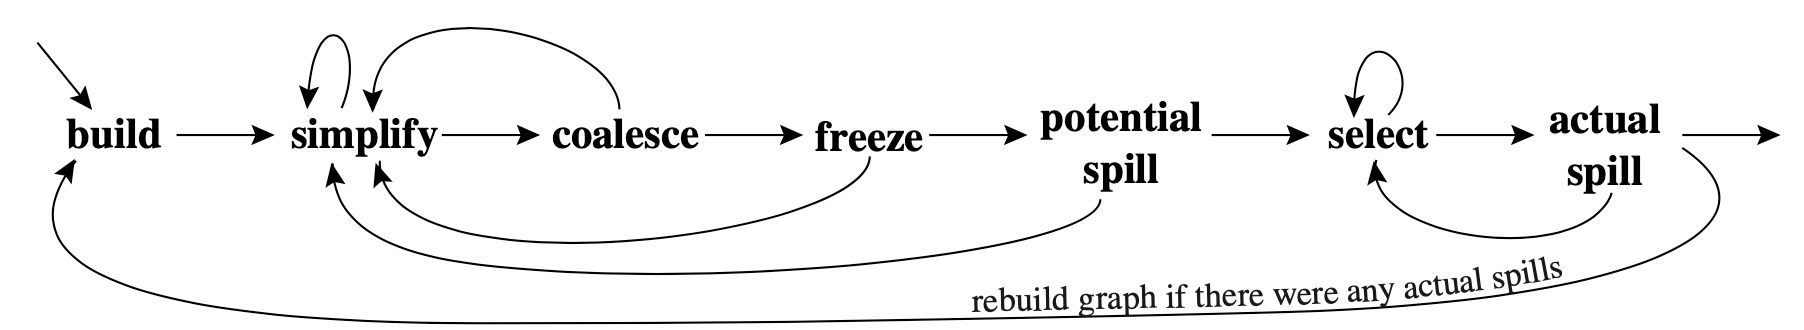
\includegraphics[width=0.8\textwidth]{regallocgraph}
  \caption{Chaitin-Briggs-George-Appel register allocation algorithm based on graph-colouring}
  \label{fig:regallocgraph}
\end{figure}

The register allocation method used is Chaitin-Briggs-George-Appel algorithm based on Kempe's graph-colouring algorithm.
Let $K$ be the number of available physical hardware register.
The steps are as can be seen from Figure~\ref{fig:regallocgraph}:
\begin{itemize}
  \item \textbf{Build}: construct the interference graph, and categorise each pseudo-register as either move-related or non-move-related.
  \item \textbf{Simplify}: one at a time, remove non-move-related nodes of low-degree ($< K$) from the graph, similar to Kempe's graph-colouring algorithm.
  \item \textbf{Coalesce}: perform conservative coalescing on the reduced graph obtained in the simplification phase.
        Conservative coalescing means that nodes are only coalesced if it will not turn a $K$-colourable graph uncolourable.
        Here we use two heuristics for conservative coalescing:
        \begin{itemize}
          \item \underline{Briggs}: two nodes can be coalesced if the resulting node will have fewer than $K$ neighbours of significant degree (having $\geq K$ edges).
          \item \underline{George}: Nodes $a$ and $b$ can be coalesced if, for every neighbour $t$ of $a$, either $t$ already interferes with $b$ or $t$ is of insignificant degree.
        \end{itemize}
  \item \textbf{Freeze}: if neither simplify nor coalesce applies, freeze all the low-degree move-related nodes -- this means that they are considered to be non-move-related, which enables more simplication.
        After this, simplify and coalesce are resumed
  \item \textbf{Potential Spill}: If there are no low-degree nodes, select a significant-degree node for potential spilling and push it on the stack.
  \item \textbf{Select}: Pop the entire stack, assigning colours if possible.
  \item \textbf{Actual spill}: If there is a node for which no colour can be applied during select, it is an actual spill.
        The program is rewritten with the spill, and the whole process is started from scratch.
\end{itemize}

Spilling priority is determined by the spilling priority score, where lower scores are more likely to be spilled.
The heuristic used is $\text{score} = (\text{number of defs and uses}) \div \text{degree}$.
This is because we want to spill variables that are least frequently defined and used, as well as those that interferes with many other variables.
Temporaries created in IR3/Lower is given higher scores than user-defined variables, and spilled temporaries are given even higher scores then temporaries created in IR3/Lower.

Note that some operands of Lower statements are actual physical hardware registers, which means that they are precoloured in terms of the graph colouring problem.
Using conservative coalescing, these registers can be coalesced with other pseudo-registers, resulting in a more optimal register allocation.
Note that care should also be taken to ensure short live-range of physical hardware registers, as they cannot be spilled into memory, unlike pseudo-registers.

Another interesting implementation is on registers \texttt{R0} to \texttt{R3} used in the calling convention.
Since they are caller-saved, their contents are clobbered after a function call.
This can be indicated in the interference graph by making these registers interfere with one another, as well as with variables that are live across function calls.
Implementation-wise, this is done by making \texttt{BRANCH\_LINK} statement use registers \texttt{R0} to \texttt{R3} and defines (clobbers) registers \texttt{R0} to \texttt{R3} as well as \texttt{R12} and \texttt{LR}.

The standard convention call is represented in Lower using \texttt{MOV} and \texttt{IMMEDIATE} statements to move the parameters into registers \texttt{R0} to \texttt{R3}, as well pushing the rest of the parameters into stack if need be, then a \texttt{BRANCH\_LINK} statement, followed by a \texttt{POP\_STACK} statement if there were parameters on the stack, and finally, a \texttt{MOV} statement to move the result of the function call to a variable if the result is used.

For example, take the following JLite statements (with the class signature in the comment):
\begin{minted}{java}
/* class Func {
 *   Func f(Int, Int, Int, Int, Int, Int); // mangled as Func_0
 *   Void g();                             // mangled as Func_1
 * }
 */
Func a; Int b; Int c; Int d; Int e; Int f;
a.f(b, 5, c, d, e, f).g();
// a, c, d, e, f are live here
\end{minted}

Lowered to IR3, the equivalent statements are:
\begin{minted}{text}
Func _t1;
_t1 = %Func_0(a, b, 5, c, d, e, f);
%Func_1(_t1);
// a, c, d, e, f are live here
\end{minted}

Lowered to Lower, the equivalent statements are:
\begin{minted}{text}
R0 <- a;     // MOV
R1 <- b;     // MOV
R2 = 5;      // IMMEDIATE
R3 <- c;     // MOV
PUSH (PAD);  // PUSH_STACK_PAD
PUSH f;      // PUSH_STACK
PUSH e;      // PUSH_STACK
PUSH d;      // PUSH_STACK
CALL Func_0; // BRANCH_LINK
POP 4;       // POP_STACK
_t1 <- R0;   // MOV
R0 <- _t1;   // MOV
CALL Func_1; // BRANCH_LINK
// a, c, d, e, f are live here
\end{minted}

Assuming that result of the register allocation is that \texttt{a} is assigned to register \texttt{R4}, \texttt{b} to register \texttt{R1}, \texttt{c} to register \texttt{R5}, \texttt{d} to register \texttt{R6}, \texttt{e} to register \texttt{R7}, \texttt{f} to register \texttt{R8}, \texttt{\_t1} to register \texttt{R0}, then the generated ARM code is:
\begin{minted}{gas}
MOV R0, R4
MOV R2, #5
MOV R3, R5
SUB SP, SP, #4
STR R8, [SP, #4]!
STR R7, [SP, #4]!
STR R6, [SP, #4]!
BL Func_0
ADD SP, SP, #16
BL Func_1
\end{minted}

Observe that \texttt{MOV} to the same registers are omitted, as this is the result of the coalescing phase done in the register allocator.
With the liveness information used to construct the interference graph, the register allocator is able to tell that variables \texttt{b} and \texttt{\_t1} do not live across function calls.
Thus, the register allocator is able to make a more optimal choice of assigning \texttt{b} to \texttt{R1}, given that it is the second parameter to \texttt{Func\_0}, while \texttt{\_t1} is assigned to \texttt{R0} as it is the first parameter of \texttt{Func\_1}.

\subsection{ARM Code Generation}
My code for the ARM Code Generation is located in \texttt{Global.java}.

With register allocation from the register allocator, the only complicated thing for ARM code generation from Lower IR is the calculation of offsets of spilled variables and stack arguments.
This is especially since the ARM calling convention specifies that stack must be 8-byte aligned, thus my compiler needs to add the appropriate padding to align the stack.

The rest of it is trivial, as most types of Lower statements correspond with exactly one ARM instruction, except for \texttt{CMP}, and comparison operators in \texttt{BINARY} and \texttt{BINARY\_BIT}.

One addition that I performed was to make the \texttt{main} function return \texttt{0}, to conform to the Unix convention.

\subsection{Optional Peephole Optimisation Passes}
There are a couple of optimisations that I have implemented for the ARM code generated.
I will expound on this in a later section.

\section{Lower IR Optimisations}
A couple of optimisations can be performed on the Lower IR.
These optimisations are run continuously until 2 runs produce the same Lower IR.

\subsection{Algebraic Identities}
The file for this is \texttt{AlgebraicPass.java}.

We make use of the following algebraic identities:
\begin{itemize}
  \item $x + 0 = 0 + x = x$ and $x - 0 = x$.
  \item $x \land true = x$
  \item $x \land false = false$
  \item $x \lor true = true$
  \item $x \lor false = x$
\end{itemize}

\subsection{Deadcode Elimination}
The file for this is \texttt{DeadcodeOptimizationPass.java}.
This optimization also makes use of live dataflow analysis implementation, located in file \texttt{LivePass.java}, and basic block analysis is located in file \texttt{FlowPass.java}.

There are a couple of dead code types that are detected in this pass:
\begin{itemize}
  \item \textbf{Basic Block}: basic blocks with in-degrees = 0 except for the entry node is removed.
  \item \textbf{Uses}: statements that defines dead variables are removed.
  \item \textbf{Dead Gotos}: delete goto statemens pointing to a label that follows the goto statement directly, i.e. \texttt{GOTO L2; L2:}, and rather use the fallthrough behaviour.
  \item \textbf{Mov to itself}: delete mov statements with the same source and destination.
  \item \textbf{Remove useless labels}: remove labels that are not the destination of any goto or if-goto statements.
  \item \textbf{Remove double goto}: remove labels whose content is another goto statement, and ensuring all gotos to the removed label go to the destination of the goto statement in the removed label.
  \item \textbf{Remove consecutive labels}: remove labels whose content is another label.
  \item \textbf{Replace label return}: Replace gotos where the destination only contains returns.
\end{itemize}

\subsection{Barrel-shifter Operand2}
Replace the sequence of \texttt{BIT} followed by \texttt{BINARY} with \texttt{BINARY\_BIT}, and \texttt{BIT} followed by \texttt{REVERSE\_SUBTRACT} with \texttt{REVERSE\_SUBTRACT\_BIT}.
If the destination of the \texttt{BIT} statement is not used anymore anywhere else, then the \textbf{Deadcode Elimination} pass will pick it up to remove the \texttt{BIT} statements.

\subsection{Constant Propagation and Constant Folding}
The file for this is \texttt{ConstantFoldingOptimizationPass.java} and \texttt{ReachingPass.java}.

Using reaching definition dataflow analysis, resolve the value of variables into a constant.
If all operands in a statement is identified, then perform constant folding: do the operation during compile time instead and turn the statement into an \texttt{IMMEDIATE} statement with the result of the operation.

This works wonderfully on the provided \texttt{test\_booleans.j} and \texttt{test\_ops.j} sample input files provided, and we are left only with print statements containing the results.

There are 2 additional passes performed on the resulting constant-propagated and constant-folded program:
\begin{itemize}
  \item \textbf{Handling large immediate}: operand2 immediate values are limited to 8-bit values rotated by an even number of bits.
        Any immediate outside of that range must be loaded from a constant pool.
        This is handled by replacing those with \texttt{LOAD\_LARGE\_IMM} Lower statement.
  \item \textbf{Inlining of println\_bool}: if the parameter to \texttt{println\_bool} is constant-folded and known at compile-time, then inline the helper function to either \mintinline{c}{puts("true");} or \mintinline{c}{puts("false");}.
\end{itemize}

\section{ARM Code Peephole Optimisations}
There are a couple of peephole optimisations that can be performed on the resulting ARM code.

\subsection{Algebraic Identities}
\subsubsection{Addition and subtraction with zero}
Replace \mintinline{gas}{ADD R0, R1, #0} or \mintinline{gas}{SUB R0, R1, #0} with \mintinline{gas}{MOV R0, R1}.

\subsubsection{And with true}
Replace \mintinline{gas}{AND R0, R1, #1} with \mintinline{gas}{MOV R0, R1}.

\subsubsection{And with false}
Replace \mintinline{gas}{AND R0, R1, #0} with \mintinline{gas}{MOV R0, #0}.

\subsubsection{Or with true}
Replace \mintinline{gas}{ORR R0, R1, #1} with \mintinline{gas}{MOV R0, #1}.

\subsubsection{Or with false}
Replace \mintinline{gas}{ORR R0, R1, #0} with \mintinline{gas}{MOV R0, R1}.

\subsection{Useless \texttt{MOV}}
Replace:
\begin{minted}{gas}
MOV R5, R0
MOV R0, R5
\end{minted}
with:
\begin{minted}{gas}
MOV R5, R0
\end{minted}

Note that we cannot remove \mintinline{gas}{MOV R5, R0} entirely as the value of \texttt{R5} might be used later on, for example, to ensure a variable survives a function call.

\subsection{Useless \texttt{LDR}}
Replace:
\begin{minted}{gas}
STR R0, [SP]
LDR R0, [SP]
\end{minted}
with:
\begin{minted}{gas}
STR R0, [SP]
\end{minted}

Note that we cannot remove \mintinline{gas}{STR R0, [SP]} entirely as that value in memory might be loaded later on.

\subsection{Remove \texttt{MOV} to itself}
Delete:
\begin{minted}{gas}
MOV R0, R0
\end{minted}

\subsection{Consecutive \texttt{MOV} of immediate values to the same register}
Replace:
\begin{minted}{gas}
MOV R0, #5
MOV R0, #1
\end{minted}
with:
\begin{minted}{gas}
MOV R0, #1
\end{minted}

\section{Additional Notes}
Possible future work includes:
\begin{itemize}
  \item Sub-expression elimination, which is probably best done on the IR3 level.
  \item Better spilling heuristic by changing the weight of the number of defs and uses inside a loop as opposed to outside a loop, for example $score = ((\text{number of defs and uses outside loops}) + 10 \times (\text{number of defs and uses inside loops})) \div \text{degree}$.
  \item Converting into Single Static Assignment form to unlock further optimisation, for example with sparse conditional constant propagation.
\end{itemize}

Just for fun, I also implemented a C backend.
The output can then be passed to any C compiler.
This can be invoked by running \texttt{./jlitec c <input file>}.

\end{document}
